%%%%%%%%%%%%%%%%%%%%%%%%%%%%%%%%%%%%%%%%%%%%%%%%%%%%%%%%%%%%%%%%%%%%
%% I, the copyright holder of this work, release this work into the
%% public domain. This applies worldwide. In some countries this may
%% not be legally possible; if so: I grant anyone the right to use
%% this work for any purpose, without any conditions, unless such
%% conditions are required by law.
%%%%%%%%%%%%%%%%%%%%%%%%%%%%%%%%%%%%%%%%%%%%%%%%%%%%%%%%%%%%%%%%%%%%

\documentclass[
  digital, %% This option enables the default options for the
           %% digital version of a document. Replace with `printed`
           %% to enable the default options for the printed version
           %% of a document.
  table,   %% Causes the coloring of tables. Replace with `notable`
           %% to restore plain tables.
  nolof,     %% Prints the List of Figures. Replace with `nolof` to
           %% hide the List of Figures.
  nolot,     %% Prints the List of Tables. Replace with `nolot` to
           %% hide the List of Tables.
  nocover
  %% More options are listed in the user guide at
  %% <http://mirrors.ctan.org/macros/latex/contrib/fithesis/guide/mu/fi.pdf>.
]{fithesis3}
%% The following section sets up the locales used in the thesis.
\usepackage[resetfonts]{cmap} %% We need to load the T2A font encoding
\usepackage[T1,T2A]{fontenc}  %% to use the Cyrillic fonts with Russian texts.
\usepackage[
  main=english, %% By using `czech` or `slovak` as the main locale
                %% instead of `english`, you can typeset the thesis
                %% in either Czech or Slovak, respectively.
  english, german, russian, czech, slovak %% The additional keys allow
]{babel}        %% foreign texts to be typeset as follows:
%%
%%   \begin{otherlanguage}{german}  ... \end{otherlanguage}
%%   \begin{otherlanguage}{russian} ... \end{otherlanguage}
%%   \begin{otherlanguage}{czech}   ... \end{otherlanguage}
%%   \begin{otherlanguage}{slovak}  ... \end{otherlanguage}
%%
%% For non-Latin scripts, it may be necessary to load additional
%% fonts:
\usepackage{paratype}
\def\textrussian#1{{\usefont{T2A}{PTSerif-TLF}{m}{rm}#1}}
%%
%% The following section sets up the metadata of the thesis.
\thesissetup{
    date          = \the\year/\the\month/\the\day,
    university    = mu,
    faculty       = fi,
    type          = bc,
    author        = Dominik Gmiterko,
    gender        = m,
    advisor       = Radek Pelánek,
    title         = {Techniques for measuring similarity of educational items},
    TeXtitle      = {Techniques for measuring similarity of educational items},
    keywords      = {similarity, measure, keyword2, ...},
    TeXkeywords   = {similarity, measure, keyword2, \ldots},
    abstract      = {This is the abstract of my thesis, which can

                     span multiple paragraphs.},
    thanks        = {These are the acknowledgements for my thesis, which can

                     span multiple paragraphs.},
    bib           = thesis.bib,
}
\usepackage{makeidx}      %% The `makeidx` package contains
\makeindex                %% helper commands for index typesetting.
%% These additional packages are used within the document:
\usepackage{paralist} %% Compact list environments
\usepackage{amsmath}  %% Mathematics
\usepackage{amsthm}
\usepackage{amsfonts}
\usepackage{url}      %% Hyperlinks
\usepackage{markdown} %% Lightweight markup
\usepackage{listings} %% Source code highlighting
\lstset{
  basicstyle      = \ttfamily,%
  identifierstyle = \color{black},%
  keywordstyle    = \color{blue},%
  keywordstyle    = {[2]\color{cyan}},%
  keywordstyle    = {[3]\color{olive}},%
  stringstyle     = \color{teal},%
  commentstyle    = \itshape\color{magenta}}
\usepackage{floatrow} %% Putting captions above tables
\floatsetup[table]{capposition=top}
\begin{document}

\newcommand{\umimeCesky}{\textit{Umíme česky}}

%
% Oficialne zadani
%
% Techniques for measuring similarity of educational items
%
% Cílem práce je prozkoumat metody pro měření podobnosti výukových položek na
% základě dat o odpovědích studentů. Práce navazuje na předchozí výzkum v rámci
% skupiny Adaptive Learning. Cílem práce je kriticky prozkoumat dříve navržené
% metody, zejména s ohledem na nevyjasněné aspekty jejich chování na reálných
% datech (neočekávané pravidelnosti v distribucích hodnot podobnosti). Na základě
% získaného vhledu budou navrženy upravené metody nebo doporučení pro praktický
% postup.
%
%                                                                   KISS
%
% „Dokonalosti není dosaženo tehdy, když už není co přidat, ale tehdy, když už nemůžete nic odebrat“ (Antoine de Saint-Exupéry)
%

\chapter*{Introduction}
\addcontentsline{toc}{chapter}{Introduction}

% --------------------------- %
% Introduction                %
% --------------------------- %

% interactive educational systems

Tutoring systems are computer-based systems designed to introduce users into various domains. They usually hold a large number of items which enables them to provide a personalized experience. To maintain this large
pool of items efficiently we need to be able to decide which items are
useful and which are not.

% focus on systems with a large number of items

% one possible method, using similarity of items

% goal of this work

% structure of this work

Besides Introduction and Conclusion chapters, this thesis is structured
into three additional chapters. First chapter talks in general about the problem of measuring similarity of educational items and advantages of using similarity.
This chapter also describes previous work and different proposed measures for computing similarity. Later we explain different types of data available in tutoring systems.
The second chapter then advances level deeper and describes observed problems specific to data we are using.
The last chapter gives an overview of many experiments that were concluded and summarizes results.

\chapter{Similarity}

% --------------------------- %
% Similarity                  %
% --------------------------- %

% Intro to chapter

%% Structure

In this chapter, we talk in general about items (questions) in tutoring systems and computing their similarity. In the beginning of the chapter we focus on better explaining basic terms like tutoring system, item, and similarity which will be used all throught the work. We also describe different kinds of data available about items and possible measures for calculating similarity.
The last section of this chapter describes data used in our experiments. In particular, we describe used dataset and outline ways of simulating artificial data.

\section{Tutoring systems}\label{tutoring-systems}

% Tutoring systems

Tutoring systems are computer systems which purpose is to teach its users (students) some knowledge or skill. These systems do this autonomously to some degree. The degree of automation may vary for each tutoring system.

%%% Autonomous aspects of tutoring systems

Many different aspects of learning may be implemented into the system or they may also be left out. The most common task which tutoring systems solve is choosing a most beneficial item from the pool of items available for users to solve. This can be done in some simple way or system may also adapt to each of the users choosing more challenging and interesting items to users who are more skilled in a specific area. While presenting users who struggle with more basic items. This is beneficial for maximizing learning aspect of the system. [CITE?] Another aspect which can tutoring systems solve is providing hints and feedback to students. When there are teachers interacting with the system we can also provide feedback about their students progress and so on.

%% Recommender systems

One closely related area are recommender systems which differ from tutoring systems only slightly. Both areas are observing users and items. The main difference is that our main source of information is a performance of users while solving specific item and recommender systems mostly use rating of the items. Which in fact are still only numbers representing slightly different things so we can still share some of the techniques. Although different goals bring different problems specific to each area.

%%% Main difference from educational systems

One difference is that we can use some additional data about items. There are item statements and solutions of students which can in some contexts give us really useful information about items.

\section{Items}\label{items}

% Items

%% Why this term

In this work, we use the term ``items'' which may refer to problems, questions, assignments in different systems. Item is a single entry in an educational system which
users can answer to. Since many aspects of this work are generally applicable we decided to use this broad term. Complexity of single item in tutoring system can differ greatly. In some tutoring systems, this may refer to simple choice from two options while in other one item is complex
tasks which user solves in a matter of minutes.

%% Data sources

To further specify the context of our research, we will describe characteristics of items. Computing similarity may be performed by different measures, but they all have to use data which are available for each item. Therefore we first describe sources of data that can be utilized for measuring the similarity of items.

\begin{itemize}
\item
  \textbf{Item statement} is some specification of the item for a learner to solve, e.g., a natural language description of the task. Another commonly used format is a grid. Many systems focusing on logic puzzles and programming problems use it.
\item
  \textbf{Item solutions} may provide us with additional information about an item. There will usually be some sample solution provided by the author and we can also utilize all the solutions from users.
\item
  \textbf{User's performance} consists of information provided indirectly by users. Performance of items may represent user solving times, correctness of the answers, number of attempts required.
\end{itemize}

Structure of both item statement and solutions differ greatly based context of tutoring system. However, in general, it is still possible to convert data into some standard form and use one of a few standard measures despite original representation.

This description of an item is broad enough to cover most of the tutoring systems. End of this chapter discusses more closely tutoring system used for our results.

%%% Tutoring systems contain educational items; the large pool is required in some contexts

The most important property of tutoring systems is that they contain educational items which are solved by users. However, amount of items in systems may vary. Some tutoring systems require a large number of items. This is especially true when they practice simple facts instead of skills. In personalized tutoring systems, the need for a large pool of items is even higher. When providing personalized questions we need a wider set of items to choose from.

%%% It may be useful to determine the similarity of items

Dealing with a large pool of items may not be easy. To maintain a pool of items efficiently we need to be able to easily decide which items are useful and which are not. One possible tool which can help us here is similarity of items.

%%% Similairty
\subsection{Measuring similarity}\label{measuring-similarity}

Following section is explaining general approach to measuring and using similarity of educational items.

% what is a similarity, how can we compute it

In general, we can compute similarity of items in many ways. We define measures for computing similarity for two items. Then when we want to use similarity for some specific use-case we compute pairwise similarities for all pair of items.

Items in our context are commonly represented as vectors of numeric values. For performance data, this is vector of correctness or time from all users to given item. Other properties of items like question statement may also be represented as a vector, e.g., by using bag-of-words.

When we have vectors for each item we can compare them pairwise to get similarity using some standard similarity measures like Pearson correlation coefficient, cosine similarity, Sokal measure or Euclidean distance.

% Edit distance

Another possible way to measuring similarity is counting edits which would convert one item to another. This is called edit distance and there are standard ways of computing it for both strings and trees. Edit distance can be then converted into similarity using something like $1 / (1 + \text{edit distance})$. So this covers another common group of information we can encounter.

% Elements of standard pipeline
\subsection{Elements of standard pipeline}\label{elements-of-standard-pipeline}

To we can wrap it up. There are a few data structures and few calculations involved in the standard pipeline for computing similarity of educational items.

\begin{enumerate}
  \item
    \textbf{Feature matrix} is matrix (items $\times$ features) containing source data. As we said previously this can represent any property of the items. This matrix consists of one vector for each item and it may represent item statement, solution or solutions of the item and naturally even users performance.
  \item
    \textbf{Measuring similarity} may involve some similarity measure or edit distance. This step is used to compute the similarity between all pairs of items. In other words, we transform feature matrix into similarity matrix.
  \item
    \textbf{Similarity matrix} is matrix (item $\times$ item) where each value represents similarity of pair of items.
  \item
    \textbf{Dimensionality reduction} is used to transform similarity matrix into a projection. Techniques like PCA or t-SNE may be used for this.
  \item
    \textbf{Projection} is more compact representation (item $\times$ 2) of similarity matrix used for visualizations for end users.
\end{enumerate}

\subsection{Why is similarity of items useful}\label{why-is-similarity-of-items-useful}

% Why is similarity of items useful
% Managing problem pool,

As we mentioned previously key part of learning is solving educational items. Defining some measures for computing similarity of items can then be used for different purposes.

First, most direct, usage is a recommendation of items for a student to solve. We do not want to recommend very similar items to those that were solved without any problems. However when user struggled system should consider recommending more of the similar problems to strengthen users knowledge.

Another possible usage is generating hints by selecting examples which are similar to the item which is currently solved. Examples are selected from a database of examples. This usage of similarity was used by [CITE Hosseini; Brusilovsky].

Two previous use cases were using problem similarity to automatically make some choices inside tutoring system. Another approach is to bring humans into the decision-making loop [CITE]. This approach provides authors of tutoring system with visualizations which should inform them what changes may be useful. E.g. detecting redundant problems and pointing out where there is not enough similar problems.

One possible way of achieving this is plotting problems to plane and displaying it to the author. This still can not be used for a very large amount of items. But we choose this approach for our specific data as they contain a large number of items but can be divided into item-sets which are solved independently in the system.

One of the use cases of visualizations is a detection of outsiders - items which behave differently than others. This behavior is directly shown in projection and such items lie far away from others.

There is one more usage of similarity which we won't be discussing further. The similarity of items can be utilized for automatic construction of clustering and hierarchical categorization. Even when author already has items categorized he can compare it to computed categorization to verify that groups are formed correctly and refine them if needed.

\chapter{Used data and techniques}\label{used-data-and-techniques}

% --------------------------- %
% Used datasets               %
% --------------------------- %

%TODO intro text
First section talks about used sources of data (dataset from actual system and simulated data).
describes structure of exercices and items intutoring system \umimeCesky{}
basic statistics can be viewed there
previous work on same dataset
Description how common projection looks like. What properties does it have
And in the end of chapter you can find detailed description of pipeline used in our experiemnts.

% types of data (real, simulated), why, real, simulated

In our analysis, we use both real data from the educational system and simulated data. Reason for this is that real-world data are useful for concluding any practical results. However, evaluation of this data is often complicated as we do not know the truth about many of its aspects. That is why we also use simulated data for validating some of our conclusions.

%% Simulated data

\section{Simulated data}\label{simulated-data}

So when simulating data we are trying to generate results which are similar to real tutoring system. However, we use slightly simpler model.

The result of the simulation consists mainly of performance matrix with items as columns and users as its rows. First, we have to generate items. For each item we choose its difficulty and skill required to solve this item. The difficulty of item is value drawn from normal distribution $\mathcal{N}(0,\,1)$.

After that, we continued with the construction of users. We generate skills for all users - a matrix of $u$ users and all used skills. This matrix is also filled with random values from normal distribution $\mathcal{N}(0,\,1)$.

Next, we simulate each user answering to each item. User answers correctly whenever is a random value higher than a logistic function of the difference of item difficulty and user skill. When it is not given answer is incorrect. User skill is one of the skills which corresponds to the skill required for given item.

We will talk more in depth about how we generated simulated data in next chapter when describing how we used them specifically. In all experiments using simulated data, we altered this basic simulation in some way to achieve results corresponding to some attribute of real data.

%% Umime cesky
\section{\umimeCesky{}}\label{umime-cesky}

%%% Czech grammar, ``fill-in-the-blank'' with two choices

\href{https://umimecesky.cz/}{\umimeCesky{}} is a system for practice of Czech grammar. The system contains multiple exercise types, but in our analysis, we use only one exercise type - simple ``fill-in-the-blank'' with two possible answers. A user is asked to choose one of them.

\begin{figure}
  
\includegraphics[width=10cm]{img/umimecesky_doplnovacka}
  \caption{``fill-in-the-blank'' example question}
  \label{fig:umimeceskydoplnovacka}
\end{figure}

Although we focused only on ``fill-in-the-blank'' exercise it can still be used to train various concepts of Czech grammar. The exercise contains many questions and they are divided into item-sets. Each item-set consists of items practicing a different aspect of language, e.g., ``Vyjmenovaná slova po B'' or ``Velká písmena: státy, oblasti''. This item-sets are arranged into hierarchical categorization as seen in the user interface. As our analysis work only with item-sets separately this categorization into different aspects is important to our work. We consider results from each item-set as it has uniform items, but we do not compare them against each other.

Items in item-sets are then divided into levels. Where higher levels are intended for solving by more experienced users as they contain more difficult questions. In general, there are three difficulty levels but not all item-sets have all three of them. Some easy item-sets include only first level. On another hand, there are item-sets which have all three levels or only higher levels.

%%% information about items: question, correctness and time

The used dataset contains multiple sources of information about items. In ``item statement'' group it is statement of the question with one missing spot and two possible answers to fill in there. We also know answers from all the users. Then in performance group of information, it is correctness of user answers and response time.

It is not possible to use response time directly. We need to normalize it in some clever way as raw response time is greatly affected by both lengths of questions and users reading speed. Also, it is a good idea to use logarithm of time instead of time itself. This is shown by [CITE]. Only then it would be useful to use data about response times. This is a reason why we are using mostly correctness of user answers.

%%% Why this system

We choose this tutoring system because, as we explained before, we are focusing on problems which are most important for systems with a large number of items. Also provided dataset has a large number of users and answers which is great for the stability of results.

%% Basic statistics
\subsection{Basic statistics}\label{basic-statistics}

\begin{table}
  \begin{tabular}{|l|r r r r|}
    \hline
     & Items & Users & Answers & Item-user answers \\
    \hline\hline
    ``Fill-in-blank'' & 6\,037 & 46\,128 & 10\,421\,521 & 7\,264\,763 \\
    \hline
    One item-set & 273 & 14\,207 & 1\,216\,403 & 888\,748 \\
    \hline
  \end{tabular}
  \caption{Basic statistics}
  \label{tab:basic-statistics}
\end{table}

This section provides some basic statistics about size of dataset and users of system. Table \ref{tab:basic-statistics} shows number of items, users and answers. Statistics are both global and for one selected item-set which is the one most commonly used for analysis. This item-set has most answers from users, therefore, it is ideal for analysis as results are more stable. We used this item-set by default but we also confirmed observed behavior on other item-sets. The last column (``Item-user answers'') contains count of unique item-user pair which are answered. This number differs from all logged answers because users can answer same item multiple times. In this case we use only one of the answers.

%%% Users using the system

A primary group of users using \umimeCesky{} are children studying at primary and secondary school. Users can have individual accounts
but system also allows teachers to create virtual class and assign students into it. Teacher is then able to select some exercises and give them to students to solve until some deadline. Each week about 200 classes visit the system.

% Previous work
\section{Previous work}\label{previous-work}

Dataset from \umimeCesky{} was used previously in few articles and thesis. Most of the work relevant to our problem comes from article Measuring Similarity of Educational Items Using Data on Learners’ Performance [CITE].

They compared few chosen similarity measures to each other. Result was that some of the similarity measures correlate greatly and some do not. It was also determined which similarity measures it is best to use for stability of results. Especially that using Pearson correlation coefficient is good default choice.

We are also using it for several reasons. Described article showed that it has good enough results in producing distinct clusters on performance data. Another reason is that Pearson correlation is easy to use as many computational environments already contain fast implementation.

Article also showed that using ``second level of similarity'' improves stability of results further. However, we choose not to use it as our dataset is large enough to be sable even with simpler measure. Using straightforward measure is also beneficial when explaining results. And this factor is important to our work.

% Description of common projection output

\section{Projection}\label{projection}

%% why is projection useful

Projections come in handy when it is hard to understand data directly because there is way too much of them. And this is our case as we focus on systems which consist of thousands of solvable items and even more users. Projections are results of dimensionality reduction techniques. We project many-dimensional data into 2 thoughtfully chosen dimensions to simplify them.

%% similarity and projection

In general we want projection which puts similar items together. This can be achieved in many different ways. Following section explains choices we made when selecting source of data, method of processing them prior to applying dimensionality reduction, and dimensionality reduction technique itself.

\subsection{Computation of item similarity}\label{computation-of-item-similarity}

%% How is projection (similarity) computed

To better understand how are projections created we have to understand steps of its computation. This is default pipeline we used in most cases. When some of the further analysis modify it slightly it is pointed out in corresponding section. Whenever we don't specify so all projections were produced using this default pipeline.

%%% Performance matrix

First step we have to take is converting raw logged information about user answers into \textbf{performance matrix}. Columns of the matrix are items in educational system and each row of the matrix contains data about single user's performance. In our case we used correctness of first users answer to specific item as his performance. This means value 1.0 in case of correct answer and 0.0 for incorrect. It is worth mentioning that performance matrix is relatively sparse as it is not common for users to solve all the items in the system.

%%% Similarity matrix

Next step is computing \textbf{similarity matrix}. It is filled with pairwise correlation of all items from performance. For this was chosen Pearson correlation coefficient based on previous work. Values produced by correlation are between $-1$ and $+1$. Each value in this matrix represent similarity of two items. This gives matrix some properties - matrix is symmetric and all values at main diagonal are 1.0.

%%% PCA, (TSNE)

The last step is producing 2D \textbf{projection}. Similarity matrix is useful for computer to directly make decision based on it. However this matrix still contains way too many values for human to interpret. As some of our goals are explaining data to users. We continue with dimensional reduction to produce more compact representation of data. This can be achieved by using any dimensional reduction technique.

%%%% PCA over TSNE

We decided to use Principal component analysis (PCA) and first two principal components are then used for 2D visualizations. We choose PCA over other commonly used technique t-SNE (which can produce better looking results) for one important reason. Results of PCA are deterministic. It produces same result for same input each time it is run. This is not true for t-SNE which is technique using machine learning and gradient descent for finding some local extreme. Stable results are more suitable for understanding data as there is no variation to results caused by algorithm. And it is much easier to compare results when altering measure used for computing item similarities.

%%% Why this pipeline, performance data (not item statement)

We choose this specific pipeline as we think it is utilizing data about items which hold most information about their similarity. Other possible choices are using item statement and solutions provided by students. However, they do not hold as much information in our specific tutoring system. Item statements in our observed exercise consist only of few Czech words with one missing spot. And student solution is only choice from two provided options. Item statement and solutions can be used more effectively in other contexts like programming, mathematics, or physics where item statements are much more complex.

This choice of pipeline is also relatively easy to understand. It consist only of few steps which can be studied separately and interchanged.

\section{Visible properties of projections}\label{visible-properties-of-projections}

% Visible Properties of projection

\begin{figure}
    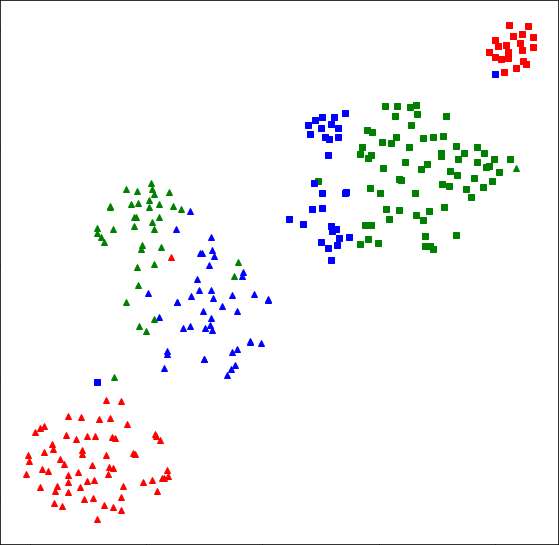
\includegraphics[width=10cm]{img/common_projection}
  \caption{Basic t-SNE projection of one item-set}
  \label{fig:common_projection}
\end{figure}

Figure \ref{fig:common_projection} shows how can resulting projection look like. This particular projection shows 273 items (single item-set). Each item is represented as one dot in the image and its proximity to others represents how similar they are.

%% Similar words near each other

As projections are meant to be used for managing item pool this puts some constrains on how ideal projection should look like.

We want similar items to end as close to each other as possible. When we use performance as data source we can also interpret as items which require same skills are projected near each other - their answers from each user correlate. For example when we look at our selected item-set we can see that all words words starting with ``bio'' are close to each other. This group consists of words witch are indeed similar because they are based on single word with added suffix. But remember, there is no information about item statement presented to similarity measure.

%% Regularities

\section{Regularities}\label{regularities}

%% This causes similar words to end-up far away one from another

After looking back at figure \ref{fig:common_projection} you can notice some regularities. Items depicted with same colors and items using same markers form clusters of same colors and markers. But so far you have no idea what this properties of items represent. This section is talking about it.

\subsection{Level regularity}\label{regularities-level-regularity}

% Level regularity
%% Description of problem, 3 clusters based on 3levels of questions difficulty

Figure \ref{fig:common_projection} contains items of three different colors. As you alread know item-sets in system \umimeCesky{} are divided into multiple levels of difficulty. For this particular item-set there are three difficulty levels. First level is depicted using red (with 110 items), second green (with 86 items), and third blue (with 77 items). You can see visible pattern in our data - each cluster consists mosly of items item from one level.

As we mentioned before, only data about user performance (correctness of answers) are used when composing projections. And there is not a direct reason for this clusters of same levels to form as no information about belonging to particular level is presented to the algorithm.

%%% cause? how users tend to solve them

Levels are not solved uniformly. It is not common for user to sole all three levels. Less experienced users tend to solve only first or first two levels. However more experienced users solve only higher levels.

%%% why is this unsuitable

%%%% Example of similar words far away one from another

This phenomenon is not suitable for analysis of item similarity as it can cause misleading results about similarity. One particular example is when similar word are displayed far away form one another just because they belong to different levels. This is visible for words ``bič'' and ``bičík'' in item set ``Vyjmenovaná slova po B''.

\subsection{Answers regularity}\label{answers-regularity}

Another property of items in figure \ref{fig:common_projection} is marker used. One type of marker (rectangle) shows items with correct answer ``i'' and another marker (triangle) shows items with correct answer ``y''. Again, there is no direct infomration about this presented to measure of similarity.

%TODO add some more general text

\chapter{Evaluation}

% --------------------------- %
% Evaluation                  %
% --------------------------- %

Chapter is explaining factors that can affect resulting projections produced from real-world data. We are focusing on higher level factors that can cause formation of clusters in projection. On low level it is apparent that items which correlate will be similar (close to each other) in projection but we focus on higher-level factors in tutoring sstems that can cause this correlation.

\section{Basic}

First section is focusing on experiments which determine range of behavior - whether distinct clusters of different answers and levels are present when altering some parameters of pipeline used to calculate projection.

\subsection{First answer vs last}

%TODO rewrite or remove
We tried using both first users answer and last in performance matrix.
However there is no visible difference in resulting projection (same
clusters are formed). This is clear when we compare first and last
answers of users. There is only 5\% difference between them. So at least
with large number of items in system it does not really matter which one
is chosen.

\subsection{Quality of clustering on different item-sets}

When introducing problem of unneeded clusters in section \ref{regularities} we showed that one particular item-set shows this behaviuor. However, we still dont know wherether this is true for all the item-sets. We decided it may be useful to quantify how recognizable are this clusters on all item-sets.

%% Quantification of level-answer clustering

Quantification of quality of clusters in the projections are executed by comparing its k-means clustering to correct level and asnwer of items. We ask k-means clustering algorithm to find \textit{levels $\times$ correct answers} clusters. Quality of clustering is then evaluated using Rand index. So value 1.0 represents that k-means divides all items into same clusters as correct classification (clusters created as combination of item level and correct answer). On other hand lover values represent it is hard to divide items correctly and there are no distinct clusters. This process is repeated multiple times to account for random initialization of k-means algorithm.

\begin{table}
  \begin{tabular}{ | l | l | l | l | }
    \hline
  	 & min & median & max \\ \hline
  	delka-samohlasek-i & 0.272173 & 0.572914 & 0.733154 \\ \hline
  	delka-samohlasek-u & 0.179007 & 0.218907 & 0.278768 \\ \hline
  	koncovky-mi-my-ma & 0.173923 & 0.378383 & 0.574999 \\ \hline
  	koncovky-ovi-ovy & -0.022328 & 1 & 1 \\ \hline
  	koncovky-podstatnych-jmen-muzsky-rod & 0.460326 & 0.526986 & 0.652672 \\ \hline
  	koncovky-podstatnych-jmen-stredni-rod & 0.444935 & 0.859304 & 0.880381 \\ \hline
  	koncovky-podstatnych-jmen-zensky-rod & 0.358566 & 0.423671 & 0.501532 \\ \hline
  	koncovky-pridavnych-jmen & 0.431434 & 0.500458 & 0.558587 \\ \hline
  	me-mne-samostatne-zajmeno-ja & -0.012182 & 0.289142 & 1 \\ \hline
  	predlozky-s-z & 0.31752 & 0.413021 & 0.455101 \\ \hline
  	psani-be-bje & -0.009319 & 0.671716 & 1 \\ \hline
  	psani-me-mne-ve-slove & 0.646219 & 0.733133 & 0.733133 \\ \hline
  	psani-nn-a-n & 0.305013 & 0.409739 & 0.462562 \\ \hline
  	psani-s-c-s-z & 0.288553 & 0.353498 & 0.44766 \\ \hline
  	psani-ve-vje & -0.013296 & 1 & 1 \\ \hline
  	shoda-podmetu-s-prisudkem & 0.189355 & 0.245732 & 0.306245 \\ \hline
  	sklonovani-zajmen-jez-jenz-nimz-ji & -0.01751 & 0.121347 & 0.353978 \\ \hline
  	slovesa-podminovaci-zvratna & 0.06066 & 0.10416 & 0.173317 \\ \hline
  	tvrde-a-mekke-souhlasky & 0.135091 & 0.257167 & 0.832182 \\ \hline
  	vyjmenovana-slova-po-b & 0.385475 & 0.597867 & 0.637596 \\ \hline
  	vyjmenovana-slova-po-l & 0.575217 & 0.641585 & 0.837544 \\ \hline
  	vyjmenovana-slova-po-m & 0.478953 & 0.928013 & 0.943975 \\ \hline
  	vyjmenovana-slova-po-p & 0.641131 & 0.832391 & 0.88884 \\ \hline
  	vyjmenovana-slova-po-s & 0.373571 & 0.421781 & 0.446662 \\ \hline
  	vyjmenovana-slova-po-v & 0.483608 & 0.678045 & 0.722796 \\ \hline
  	vyjmenovana-slova-po-z & 0.528562 & 0.565708 & 0.657444 \\ \hline
  \end{tabular}
  \caption{Quality of clusters in different item-sets}
  \label{tab:quality-of-clusters}
\end{table}

Table \ref{tab:quality-of-clusters} describes quality of clusters on different item-sets. Results show that many item-sets have distinct clusters of different levels and answers. But there are some item-sets with obscure structure of projection. This mostly occurs when item-set have large number of possible answers.

% Why we are looking at both item-answer clusters and not separated?

We were looking at both clusters of answers and levels simultaneously. Another possible choice would be to somehow quantify both quality of levels and answers separately but this straightforward approach would not work there. Simplest example showing why would consists of two levels and two correct answers - where correct answers are divided evenly in each level. When we ask k-means to create two clusters for levels and two clusters for answers it will return same clustering in both cases because number of clusters is only used parameter. This will result in one metric returning high value but other one small even when clusters are really distinct.

% Conclusion

So we can conclude that this behavior is present in all item-sets.

%%% Different similarity measures

\subsection{Different similarity measures}

In another experiment we inter exchanged four different measures for computing similarity of items to verify that previous results aren't specific to single measure. Especially whether they all preserve smaller similarity of items with different levels and correct answer.

\begin{figure}
  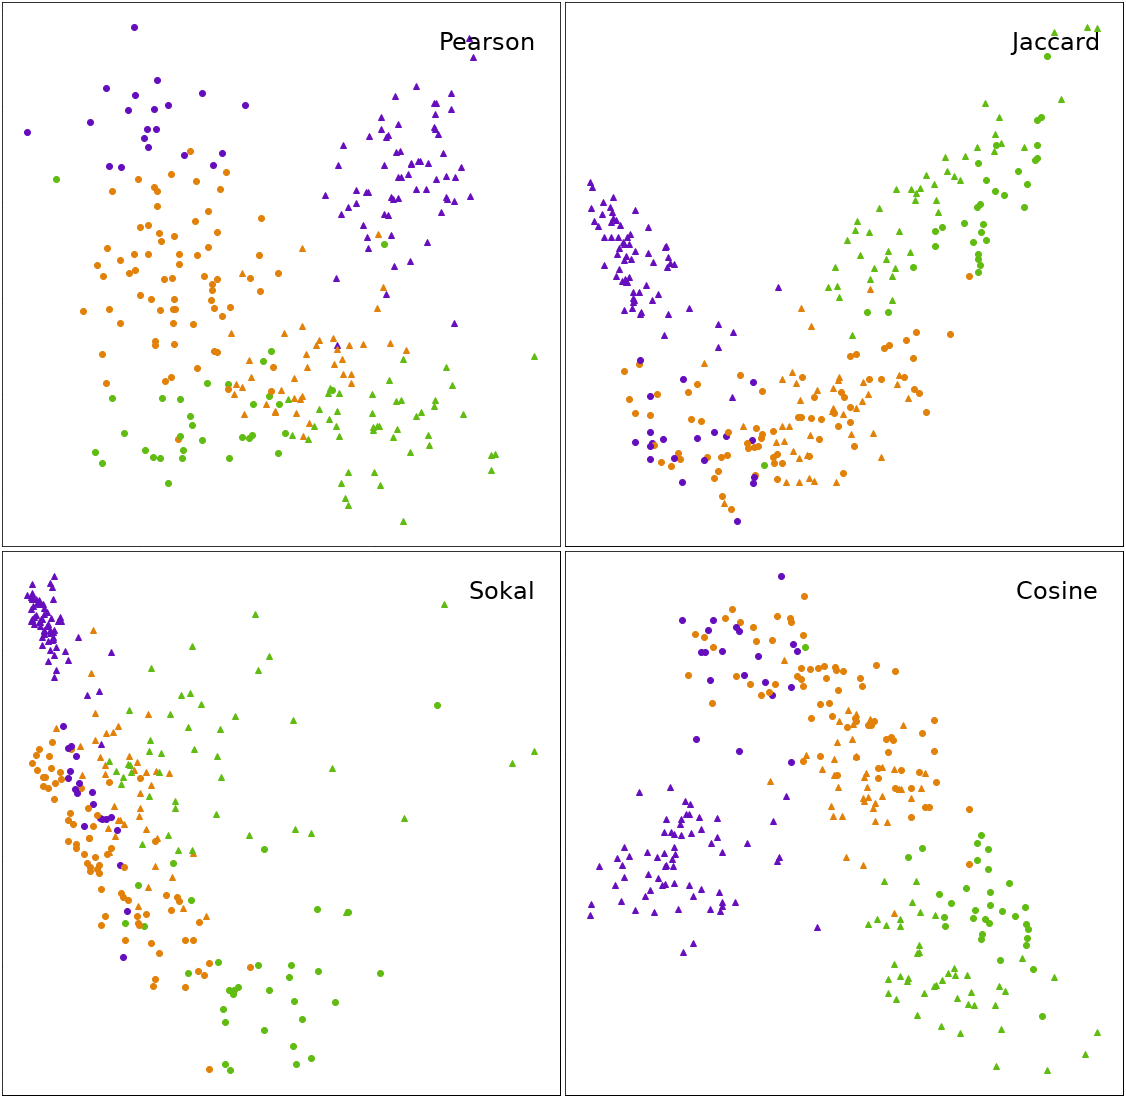
\includegraphics[width=10cm]{img/measures}
  \caption{Comparison of four similarity measures}
  \label{fig:measures}
\end{figure}


% preserving of clusters

Figure \ref{fig:measures} shows four different similarity measures used on same data. Resulting projections are different. However, they all preserve information which is causing items from same level and answer to form clusters. Different colors represent different levels and markers different answers.

% What different measurements measure

When we encounter performance matrix which contains only two (boolean) values, we can summarize performance of all users on items $i$ and $j$ by using just four values. See table \ref{tab:boolean-attributes}.

\begin{table}
  \begin{tabular}{ l | l | l | }
  \hline
  	 & incorrect & correct \\ \hline
  	incorrect & $a$ & $b$ \\ \hline
  	correct & $c$ & $d$ \\ \hline
  \end{tabular}
  \caption{Attributes of boolean similarity measures}
  \label{tab:boolean-attributes}
\end{table}

\begin{itemize}
\item
  \textbf{Pearson} ($(ad - bc) / \sqrt{(a+b)(a+c)(b+d)(c+d)}$) is commonly used. It correlates well with much simpler measure \textbf{Yule} ($(ad-bc)/(ad+bc)$).

\item
  \textbf{Jaccard} differs visibly from other measures.

  %TODO !!!!!!!!!!!!!!!!!!!!!!!!
  Similarity of items is not greater in one group of questions (based on correct answer).

  Similarities provided by Jaccard measure differe greatly from other
  measures. Resulting projection still shows same clusters of level and
  items are splited based on correct answer but information is kept in
  another way than in correlation based measures like Pearson.

\item
  \textbf{Sokal} shows best that different similarity measures can highlight different aspects of item performance. Similarity of items  heavily depends on performance of items when using Sokal. (Where performance of item is amount of correct answers divided by all answers.) Items with higher performance are much more similar than items with lower performance. This is causing packed cluster of items from first level (easy) and spread out cluster of items from third level (harder).

\item
  \textbf{Cosine} similarity produces projection similar to Jaccard.
\end{itemize}

cluseters are preserved

So we can conslude that this bahaviour is present despite of used similarity measure.

\section{Answers regularity}

\subsection{Total similarity histogram}





\subsection{Performance matrix}

what can one answer possibly affect in different matrices



\subsection{Simulated default answer}





\subsection{Filter out users}





\section{Levels regularity}

\subsection{Simulate missing data}





\subsection{Item performance}




















\section{Level regularity}\label{level-regularity}

\subsection{Sparseness of performance
matrix}\label{sparseness-of-performance-matrix}

%% question? can missing data affect result of similarity calculation

%%% Simulated data experiment

In same way as we explained before in section ??. Only difference is that resulting performance matrix will now contain missing values. We wanted to recreate missing data in similar way that this occurs in real performance matrix. This is achieved by simulated users not solving all items. Each user starts with solving one level and then with some probability continues to another. So most users solve only one level, some users solve 2 levels and only few users solve all 3 levels. Order in which they answer levels is chosen at random as users are not required to continue chronologically. This is also visible in real data - there are users who solve only second or only highest difficulty level.

Results indicate that that structure of data can affect results only in really special cases. The only case where projection is divided into clusters is when there is absolutely no information between question in different levels. But this is not our case in real data as there are users solving multiple levels.

%% Users similarity

\section{Users similarity
projection}\label{users-similarity-projection}

Insead we choose to analyse whether our data contains different groups
of users. We are changing how we are looking at data.Up until now we
used item-item similarity to calculate projection of items. Now we are
going to to be using user-user similarity.

It is worth mentioning we will work with larger matrices as this forced
us to do some optimizations in code of our analysis. For example
similariy matrix of items usualy has size between $100\times 100$ and
$300\times 300$. As we are looking only on items from single knowledge
component. Hovewer user similarity matrix is square matrix with size
around $10 000\times 10 000$. This is also reason why current
recommender systems use item similarity instead of user similarity. CITE

First attempt on projecting users can be seen in figure ??.

% TODO users similarity img

We say that user solved level when he answered at least 30 questions
(which is 1/3 of questions for observed item set). Based on this we can
divide users into 8 groups. We added color to each group so we can
distinguish them in following plots easily.

\begin{table}
  \begin{tabular}{ | l | l | l | l | }
  \hline
  	Group & Color & Users \\ \hline
  	none & black & 35\% \\ \hline
  	only 1st level & red & 31\% \\ \hline
  	only 2nd level & green & 9\% \\ \hline
  	only 3rd level & blue  & 8\% \\ \hline
  	both 1th and 2nd & yellow & 7\% \\ \hline
  	both 2nd and 3rd & cyan & 2\% \\ \hline
  	both 1nd and 3rd & magenta & 2\% \\ \hline
  	all levels & light gray & 7\% \\ \hline
  \end{tabular}
  \caption{Groups of users}
  \label{tab:groups}
\end{table}


We can see that all formed clusters of users contains in most cases users
from single user group when we divide them by levels they solved. This
brought us to more interesting discoveries. In general each level and
each item has some mean performance. This is shown in figure ??.
Horizontal axis contains items sorted by level and mean performance.
Vertical axis shows performance of each item. Given item sets have mean
performance 94\%, 86\%, 71\% for each level respectively.

After dividing users into 8 groups plot changes slightly. Some groups
like ``only 1st level'' (its colored red and contains users who solved
primarily first level and only few or none items from other levels) has
much lower performance on other levels. We can conclude that users who
tend to solve mostly first level are not as experienced as other users. On
other hand users in group ``both 2nd and 3rd'' (cyan) are performing
better than other users on all three levels.

At this point we have to return to simulation. We want to show that
grouos of users solving levelswith different performancecan cause
forming of clusters of items from same level.

Answers are simulated pretty mutch same as in previous simulated
experiments. We have 300 items divided into 3 levels. There is 3000
simulated users. Most of them solve levels with same skill but some 1/5
of users have smaller chance to solve second and third level. This is
visible on item performance polt similar to one from real data.

Only chnged variable was performance of some users for levels and this
resulted in visible clusters in projection (figure ??).

From otained information we can conclude that removing subnormal answers
of users (few answers to other levels when they solved primarly one
level) should remove clusters of levels.

But does it?!?

\section{Answer regularity}\label{answer-regularity}

% Answer regularity
%% Description of problem, items are divided into
clusters based correct answer (i/y) when there is no information about
this in data used for computing similarity

%%% TODO Outsider detection using similarity data

When exploring data, it may be useful to detect outsiders. It may be
useful for multiple reasons [CITE]. In our particular case we
declare item an outsider when it is not similar to any other items in
item set. seems like a logical path to take.

In particular this means item with low sum of similarities to other
items may be an outsider. This is where we encountered another
regularity in data.

%% Total similarity

Sum of similarities is sum of one column of similarity matrix which we
produced in our workflow for computing projection.

\begin{figure}
  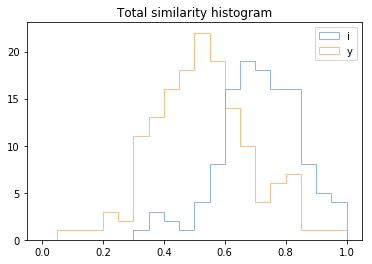
\includegraphics[width=10cm]{img/histogram_i_y}
  \caption{Histogram of similarities}
  \label{fig:histogram_i_y}
\end{figure}

%%% total similarity histograms by answer

%%% quantification for different concepts

This is not specific to only one problem set (which was used in previous
images), almost all problem sets display similar pattern. However for
some its more distinct than for others. (Sets consisting of items with
many possible answers do not behave this way. But that is to be
expected.)

%% Users are choosing one answer by default when they do not know answer

Our next experiment was simulation of users preferring one answer in
case they do not know what is the correct answer.

Answers are simulated for each user and question. There are no missing
values. Answer is correct whenever random value is higher than logistic
function of (users skill) - (difficulty of question). Half of questions
has one correct answer and other half another answer. We used this to
shift chance of answering correctly higher or lower (+0.1 for first
answer and -0.1 for second).

%\includegraphics{simulated_projection.png}
%\includegraphics{simulated_correlation_similarity_performance.png}

Colors represent answer of each item (chance shifted up or down). There
are formed visible clusters of same answers in result similar to
real-wold data. Using two uncorrelated skills cause clusters in
projection. (When using only single skill for all questions results does
not change and they are not required for this simulation.)

%%% it is usually answer on left, but there are exceptions koncovky
pridavnych mien je to Y (v pravo)

This is not specific to only one category (which was used in previous
images), many more categories display similar pattern. However for some
its more distinct than for others. For some distribution of similarities
is same for all answers (psani-nn-a-n, vyjmenovana-slova-po-p,..).

We picked few witch have very distinct clusters of answers and looked whether it is
answer on left or on right in user interface. Our finding was that not all concept prefer answer which is  located

%%% how to detect this in performance data? / what can we detect in
data?

%% Division of user answers 50-50, but not for correct answers

We observed before that whole data set uses both answers the same but
for single user this may not be true. There are even users who use only
one answer as seen in following performance matrix. There is a line with
all questions answered incorrectly for one answer and correctly for
another.

%\includegraphics{uneven_answers_perforamnce_perf_matrix.png}

We can filter this users out. Next three images show different levels of
filtering. First uses no filtering at all (uses all users). Second and
third image filter users by difference between performance on each
answer. (So if users has same performance on question with both answers
this value is 0.0 and when user uses only one of the answers (biggest
possible difference) value is 1.0). Second image shows value of 0.3
(performance on one answer is 30% higher than on the other one). And
third image uses value 6% which is median.

%\includegraphics{uneven_answers_perforamnce_none.png}
%\includegraphics{uneven_answers_perforamnce_0_3.png}
%\includegraphics{uneven_answers_perforamnce_half.png}

When we use only half of users which have uniform answers there are no
clusters of question with same answers. (Half of users because median is
used as filtering value.)

We can look at histogram of difference between answers. For most of the
users there is almost no difference but there are users with higher
difference in performance between answers.

%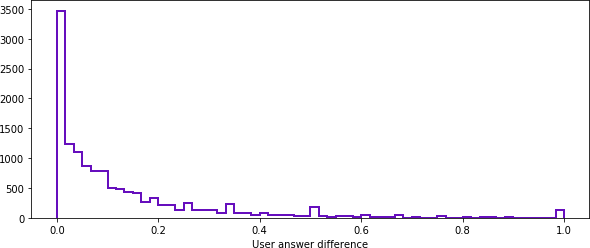
\includegraphics{uneven_answers_hist.png}

I look at difference between performance (amount of correctly answered
questions) instead of usage of each answer because it is performance
that affects calculated similarity of questions. However they should
correlate somewhat. Another reason is that it is closer to simulated
experiment so we can compare results directly.

When we simulated users we gave them all habit to use one answer more
commonly. But not all users have this habit in real-wold data. However
there is quite large amount of users who do.

This resolves first problem we encountered but does not explain other
regularities in data.

%%% Simulation of default answer
\subsection{Simulation of default answer}\label{simulation-of-default-answer}

This next simulation is also using same core but is enhanced with further choosing correct answer for each item. This is used to offset logistic function higher or lower to simulate higher chance of succeeding in solving items with correct answer is the users preferred one. We think this is good enough solution to simulating users choosing one answer by default when they are unsure about answer.

This specific simulation is using two uncorrelated skills and two answers. They are distributed in a way that there is same amount of each combination (1/4 of items). From previous work we know that uncorrelated skills will form distinct clusters. We included them in this simulation to better illustrate conditions of real data - as such clusters of levels exist there.

Projection of data simulated in this way has same properties as our real data. There are clusters (in this case caused by uncorrelated skills) which have items divided by correct answer.

%TODO better reasoning for this, explain why this happends
	% why does data simulated in this way project to clusters of levels and answers

We succseeded in simualting data with clusters of same answers and
showing that this is case in our real data. Hovewer there is still one
more thing to explain - clusters of uqesrions with same levels.
Folloving same approach we can try to filter out users with large
difference in how successfuk they are with solving different levels.

Weused histogram of differences (variance of solved levels) to choose
some value for filtering of users. As more than half of users solves
only one level median of differences is 0.0. So we choose one value just
by looking at histogram. We can see in following figure that this dosnt
really matter as filtering users in this way does not help with
eliminating clustrs of same levels.

%TODO this is enought to normalize resulting projection so it has good properties
% % TODO check gradient of performance, is it good
% % similar items from different levels are closer to each other


\section{User similarity}\label{user-similarity}

% User similarity

For explaining patterns of aquestions from same level we have to dig
deeper and understand different fpgroups of users. One particular way
how to acjive this is using owrkflow similar to previous. Althought
there will be one difference, we will be using similarity of users
instead of items. (item-item similarity matrix, user-user similarity
matrix). This also meqns that we have to transpose performance matrix -
so each column represents one user. Calculating correlarion between all
columns gives us user similarity matrix. There is no difference in
projection step, only used matrix is interexchnaged.

W pe ca.n try ploting this result direcly using PCA. Hovewer we would
notice that resulting image doesnt give us much information about users.
reason for this is that two principal components reflect some property
of data that we know about and dont wqnt to display. In particular users
solving only one group are somewhat special. Columns representing users
like this cannot be compared when they solved different levels - there
is missinf information about their correlarion. PCA chooses this
information with highest magnitude In presented figure this coresponds
to choosen components reflecting solving of first and third level.
(third principal domponent is corelates with solving of second level)

As users who solve only one level cause this behaviour. And they dont
give us information about similarity of items in different levels we
choose to exclude this users. After doing so we end up with projection
similar to figure xx.

There are two visible clusters of users. Futher analysis shows that
difference beween groups of users is caused by ?

\section{Another contexts}\label{another-contexts}

%% (re)Usage in other concepts

%% Explain my idea of how can data affect projection -> possible affected items from one performance value

\chapter{Conclusion}

% --------------------------- %
% Conclusion                  %
% --------------------------- %

We can conclude some recommendations. While trying to explain patterns
in our particular used data we run into multiple situatutions hwich can
repeat even when explaing some different data using similalr techniques.


determining range of effect.. its stupidly simple, but can be forgotten whenfacig some problem and may help you greatly


Technique we used for calculating projections is quite common in area of
Adaptife learning and recommender systems. CITE.

% Problems specific for dataset may arise

Following section will summarize recommendations useful for explaining
results

it is useful to look at both item and user similarity - some
patterns in data can be results of habbits of users. - we are using
unsupervsed learning like techniques - we obtain some results but it is
hard to explain why they are like they are.. one possibility how to
explain results is using simulations - we explained one possible way of
simulating performance matrix - data fome from users so identifing
groups of users who behave same may be useful - we rhink most common
groups which can be vosibke in data coming from online tutoring system
are eager users and trolls - Main grohp of users tend to answer to
quesrions in some regullar patrern based on their knowledge while trolls
follow different pattern (for exampla use same answer on all questions)
- looking at total similarity of items - typicaly correlates with first
dimension of PCA - variance of performance entries of items

% Now we understand how structure of system may affect performance data

% Reusable in other systems

% Limitations
\section{Limitations}\label{limitations}

- only one exercise
- only performane was used for computing similarity of items, other sources of data were ignored .. as we thought there results here are most unexpected .. hovewer there may arise other problems when using different sourcess of data
- we used only correctness of answers and ignore response time. It make sense in studied tutoring system but may be important in other systems.


  \makeatletter\thesis@blocks@clear\makeatother
  %\phantomsection %% Print the index and insert it into the
  %\addcontentsline{toc}{chapter}{\indexname} %% table of contents.
  %\printindex

\appendix %% Start the appendices.
\chapter{An appendix}
Here you can insert the appendices of your thesis.

\end{document}
